\documentclass[12pt,letterpaper]{article}
\usepackage[utf8]{inputenc}
\usepackage[spanish]{babel}
\usepackage{amsmath}
\usepackage{amsfonts}
\usepackage{amssymb}
\setlength{\parindent}{0pt}
\setlength{\parskip}{0em}

%Para agregar paquetes adicionales, colocar coma y agregar:
\usepackage{latexsym, amssymb, amsmath, amsthm, color, asymptote, graphicx, fancyhdr, caption, cancel,multicol}

%Punto Decimal
\decimalpoint

%Parte entera
\providecommand{\myfloor}[1]{\left \lfloor #1 \right \rfloor }
\providecommand{\myceil}[1]{\left \lceil #1 \right \rceil }
\providecommand{\mypar}[1]{\left( #1 \right) }
\providecommand{\mycor}[1]{\left[ #1 \right] }

%Abreviaciones
\newcommand{\N}{\mathbb{N}}
\newcommand{\C}{\mathbb{C}}
\newcommand{\R}{\mathbb{R}}
\newcommand{\Q}{\mathbb{Q}}
\newcommand{\Z}{\mathbb{Z}}

%Tricks
\usepackage{pgf,tikz}
\usepackage{mathrsfs}
\usetikzlibrary{arrows}
\usetikzlibrary{babel}

%usepackage{pstricks-add}

%Para modificar los márgenes del documento:
\usepackage[paper=letterpaper,right=2.5cm,left=2.5cm,top=1.5cm,bottom=1.5cm]{geometry}


\theoremstyle{definition}
\newtheorem{ejemplo}{Ejemplo}[section]
\newtheorem{defi}{Definición}[section]
\newtheorem{problem}{Problema}[section]
\newtheorem{ejer}{Ejercicio}[section]
\setcounter{section}{0}

\theoremstyle{plain}
\newtheorem{conj}{Conjetura}[section]
\newtheorem{teo}{Teorema}[section]
\newtheorem{colo}{Corolario}[section]
\newtheorem{lema}{Lema}[section]
\newtheorem{propo}{Proposición}[section]

\theoremstyle{remark}
\newtheorem{obser}{Observación}[section]

%Hacer cálculos matematicos
\usepackage{expl3, xparse}
\ExplSyntaxOn
\DeclareDocumentCommand { \myformat }{m}
  { \fp_to_decimal:n { round((#1),9) } }
\ExplSyntaxOff

%Simbolos matemáticos
\newcommand{\ndiv}{\hspace{-4pt}\not|\hspace{2pt}}

\usepackage{tcolorbox}
\tcbuselibrary{theorems}
\newtcbtheorem[number within=section]{mytheo}{Teorema}%
{colback=green!5,colframe=green!35!black,fonttitle=\bfseries}{th}

\newtcbtheorem[number within=section]{mydefi}{Definición}%
{colback=red!5,colframe=red!35!black,fonttitle=\bfseries}{th}

\usepackage{listingsutf8}
\usepackage{listings}
\usepackage{color} %red, green, blue, yellow, cyan, magenta, black, white
\definecolor{mygreen}{RGB}{28,172,0} % color values Red, Green, Blue
\definecolor{mylilas}{RGB}{170,55,241}

\usepackage{algpseudocode}

\begin{document}
\author{Ricardo Largaespada}
\title{Métodos Numéricos - Laboratorio 1}
\date{13 de marzo de 2025}
\maketitle

\lstset{language=Matlab,%
    %basicstyle=\color{red},
    breaklines=true,%
    morekeywords={matlab2tikz},
    keywordstyle=\color{blue},%
    morekeywords=[2]{1}, keywordstyle=[2]{\color{black}},
    identifierstyle=\color{black},%
    stringstyle=\color{mylilas},
    commentstyle=\color{mygreen},%
    showstringspaces=false,%without this there will be a symbol in the places where there is a space
    numbers=left,%
    numberstyle={\tiny \color{black}},% size of the numbers
    numbersep=9pt, % this defines how far the numbers are from the text
    emph=[1]{for,end,break},emphstyle=[1]\color{red}, %some words to emphasise
    %emph=[2]{word1,word2}, emphstyle=[2]{style},    
    literate=%
         {á}{{\'a}}1
         {í}{{\'i}}1
         {é}{{\'e}}1
         {ú}{{\'u}}1
         {ó}{{\'o}}1
         {Á}{{\'A}}1
         {Í}{{\'I}}1
         {É}{{\'E}}1
         {Ú}{{\'U}}1
         {Ó}{{\'O}}1
}

\section{Método de Bisección}
El método de bisección, conocido también como de corte binario, de partición de intervalos o de Bolzano, es un tipo de búsqueda incremental en el que el intervalo se divide siempre a la mitad. Si la función cambia de signo sobre un intervalo, se evalúa el valor de la función en el punto medio. La posición de la raíz se determina situándola en el punto medio del subintervalo, dentro del cual ocurre un cambio de signo. El proceso se repite hasta obtener una mejor aproximación.

\subsection{Criterios de paro y estimación de errores}
Una sugerencia inicial sería finalizar el cálculo cuando el error verdadero se encuentre por debajo de algún nivel prefijado. Dicha estrategia es inconveniente, ya que la estimación del error en el ejemplo anterior se basó en el conocimiento del valor verdadero de la raíz de la función. Éste no es el caso de una situación real, ya que no habría motivo para utilizar el método si se conoce la raíz.\\

Por lo tanto, se requiere estimar el error de forma tal que no se necesite el conocimiento previo de la raíz. Se puede desarrollar una formulación alternativa en la aproximación del error relativo porcentual
\begin{align}
\varepsilon_a=\left|\frac{x_u-x_l}{x_u+x_l}\right|100\label{eq:10}\% 
\end{align}

Aunque el método de bisección por lo general es más lento que otros métodos, la claridad del análisis de error ciertamente es un aspecto positivo que puede volverlo atractivo para ciertas aplicaciones en ingeniería.\\

Otro beneficio del método de bisección es que el número de iteraciones requerido para obtener un error absoluto se calcula a priori. Debido a que en cada iteración se reduce el error a la mitad, la fórmula general que relaciona el error y el número de iteraciones, $n$, es $$E_a^n=\frac{\Delta x^0}{2^n}.$$
Si $E_{a,d}$ es el error deseado, en esta ecuación se despeja \begin{align}
n=\log_2\mypar{\frac{\Delta x^0}{E_{a,d}}}
\end{align}

\subsection{Algoritmo de Bisección}

El siguiente programa tiene en cuenta los siguientes aspectos: 
\begin{itemize}
\item En caso que no se defina una tolerancia (error absoluto), el programa utilizará una por defecto.
\item Si no se define la variable {\bf filter}, que funciona para saber si en el intervalo dado exista una singularidad (esto es, que haya más de una raíz en el intervalo), el programa no lo considerará.
\end{itemize}

\lstinputlisting{codes/bisect.m}

\newpage

\begin{ejemplo}
Dada $$f(x)=-2x^6-1.5x^4+10x+2$$ Use el método de bisección para determinar el {\it máximo} de esta función. Haga elecciones iniciales de $x_l=0$ y $x_u=1$, y realice iteraciones hasta que el error relativo aproximado sea menor que $5\%$.
\end{ejemplo}
{\it Solución.} Primero tengamos en cuenta que para encontrar el máximo de una función, debemos utilizar el criterio de la segunda derivada y evaluar si $f''(a)$ es mayor que $0$, donde $a$ es un número crítico. Así pues encontremos los números críticos de $f$, estos cumplen que: $$f'(x)=-12x^5-6x^3+10=0.$$

Modificando el algoritmo de bisección anterior para que este se detenga hasta que $e_a$ sea menor a $5\%$.

\lstinputlisting[language=Matlab]{codes/bisectej1.m}

El número crítico se obtiene al evaluar: 
\lstinputlisting{codes/lab2_ejemplo1.m}
Obteniendo así: $root = 0.84375$, de donde el máximo valor de $f(x)$ es: $8.955640656873584$.

\newpage 

\section{Método de la Falsa Posición}
Aún cuando la bisección es una técnica perfectamente válida para determinar raíces, su método de aproximación por ``fuerza bruta'' es relativamente ineficiente. La falsa posición es una alternativa basada en una visualización gráfica.\\

Un inconveniente del método de bisección es que al dividir el intervalo de $xl$ a $xu$ en mitades iguales, no se toman en consideración las magnitudes de $f(x_l)$ y $f(x_u)$. Por ejemplo, si $f(x_l)$ está mucho más cercana a cero que $f(x_u)$, es lógico que la raíz se encuentre más cerca de $x_l$ que de $x_u$. Un método alternativo que aprovecha esta visualización gráfica consiste en unir $f(x_l)$ y $f(x_u)$ con una línea recta. La intersección de esta línea con el eje de las $x$ representa una mejor aproximación de la raíz. El hecho de que se reemplace la curva por una línea recta da una ``falsa posición'' de la raíz; de aquí el nombre de {\it método de la falsa posición}, o en latín, {\it regula falsi}. También se le conoce como {\it método de interpolación lineal}.\\

Usando triángulos semejantes, la intersección de la línea recta con el eje de las $x$ se estima mediante \begin{align}
\frac{f(x_l)}{x_r-x_l}=\frac{f(x_u)}{x_r-x_u}
\end{align}
en el cual se despeja $x_r$ \begin{align}
x_r=x_u-\frac{f(x_u)(x_l-x_u)}{f(x_l)-f(x_u)} \label{eq:3}
\end{align}
Ésta es la fórmula de la falsa posición. El valor de $x_r$ calculado con la ecuación (\ref(eq:3)), reemplazará, después, a cualquiera de los dos valores iniciales, $x_l$ o $x_u$, y da un valor de la función con el mismo signo de $f(x_r)$. De esta manera, los valores $x_l$ y $x_u$ siempre encierran la verdadera raíz. El proceso se repite hasta que la aproximación a la raíz sea adecuada.

\subsection{Algoritmo de la falsa posición}
\begin{multicols}{2}
\begin{algorithmic}[1]
\Function{FalsePos}{xl, xu, es, imax, xr, iter, ea}
\State{iter = 0}
\Repeat
\State{xrold=xr}
\State{xr=xu$-$f(xu)*(xl$-$xu)/(f(xl)$-$f(xu))}
\State{iter=iter$+$1}
\If{xr$<>$0}
\State{ea=ABS((xr$-$xrold)/xr)*100}
\EndIf
\State{test=f(xl)*f(xr)}
\If{test$<$0}
\State{xu=xr}
\ElsIf{test$>$0}
\State{xl=xr}
\Else
\State{ea=0}
\EndIf
\Until{ea$<$es OR iter $\ge$ imax}
\State{FalsePos = xr}
\EndFunction
\end{algorithmic}
\end{multicols}

\newpage

\section{Búsqueda por Incrementos y Determinación de Valores Iniciales}
Además de verificar una respuesta individual, se debe determinar si se han localizado todas las raíces posibles. Como se mencionó anteriormente, por lo general una gráfica de la función ayudará a realizar dicha tarea. Otra opción es incorporar una búsqueda incremental al inicio del programa. Esto consiste en empezar en un extremo del intervalo de interés y realizar evaluaciones de la función con pequeños incrementos a lo largo del intervalo. Si la función cambia de signo, se supone que la raíz está dentro del incremento. Los valores de $x$, al principio y al final del incremento, pueden servir como valores iniciales para las técnicas descritas en esta clase.\\

Un problema potencial en los métodos de búsqueda por incremento es el de escoger la longitud del incremento. Si la longitud es muy pequeña, la búsqueda llega a consumir demasiado tiempo. Por otro lado, si la longitud es demasiado grande, existe la posibilidad de que raíces muy cercanas entre sí pasen inadvertidas. El problema se complica con la posible existencia de raíces múltiples. Un remedio parcial para estos casos consiste en calcular la primera derivada de la función $f'(x)$ al inicio y al final de cada intervalo. Cuando la derivada cambia de signo, puede existir un máximo o un mínimo en ese intervalo, lo que sugiere una búsqueda más minuciosa para detectar la posibilidad de una raíz.\\

Aunque estas modificaciones o el empleo de un incremento muy fino ayudan a resolver el problema, se debe aclarar que métodos tales como el de la búsqueda incremental no siempre resultan sencillos. Será prudente complementar dichas técnicas automáticas con cualquier otra información que dé idea de la localización de las raíces. Esta información se puede encontrar graficando la función y entendiendo el problema físico de donde proviene la ecuación.\\

A continuación un algoritmo desarrollado en Matlab que permite encontrar la menor raíz (si existe) en un intervalo cerrado de una función.

\lstinputlisting{codes/rootsearch.m}

\newpage

\section*{Problemas Propuestos}

\begin{multicols}{2}
{\problem Determine las raíces reales de $f(x) = -0.5x^2 + 2.5x + 4.5$:\begin{itemize}
\item[a)] Gráficamente
\item[b)] Empleando la fórmula cuadrática
\item[c)] Usando el método de bisección con tres iteraciones para determinar la raíz más grande. Emplee como valores iniciales $x_l = 5$ y $x_u = 10$. Calcule el error estimado $e_a$ y el error verdadero $e_t$ para cada iteración.\end{itemize}}

{\problem Determine la raíz real de $\ln{(x^2)}=0.7$:\begin{itemize}
\item[a)] Gráficamente
\item[b)] Empleando tres iteraciones en el método de bisección con los valores iniciales $x_l = 0.5$ y $x_u = 2$.
\item[c)] Empleando tres iteraciones del método de la falsa posición, con los mismos valores iniciales de b).
\end{itemize}}

{\problem Encuentre la raíz positiva más pequeña de la función $x^2|\cos{\sqrt{x}|}=5$ usando el método de la falsa posición. Para localizar el intervalo en donde se encuentra la raíz, grafique primero esta función para valores de $x$ entre $0$ y $5$. Realice el cálculo hasta que $\epsilon_a$ sea menor que $\epsilon_s=1\%$. Compruebe su respuesta final sustituyéndola en la función original.}

{\problem La velocidad $v$ de un paracaidista que cae está dada por $$v=\frac{gm}{c}\mypar{1-e^{-(c/m)t}}$$ donde $g=9.81\,m/s^2$. Para un paracaidista que con coeficiente de resistencia de $c=15\,kg/s$, calcule la masa $m$ de modo que la velocidad sea $v=36\, m/s$ en $t=10\,s$. Utilice el método de la falsa posición para determinar $m$ a un nivel de $\epsilon_s=0.1\%$.}

{\problem Use bisección para determinar el coeficiente de resistencia necesario para que un paracaidista de $82\,kg$ tenga una velocidad de $36\,m/s$ después de $4\,s$ de caída libre. Comience con valores iniciales de $x_l=3$ y $x_u=5$. Itere hasta que el error relativo caiga por debajo de $2\%$.}

{\problem Suponga que está diseñando un tanque esférico (ver figura) para almacenar agua para un poblado pequeño en un país en desarrollo. El volumen del líquido que se puede contener se calcula con $$V=\pi h^2\frac{[3R-h]}{3}$$ donde $V=$ volumen [$m^3$], $h=$ profundidad del agua en el tanque [$m$] y $R=$ radio del tanque [$m$].\\
Si $R=3\,m$, ¿a qué profundidad debe llenarse el tanque de modo que contenga $30\,m^3$? Haga tres iteraciones con el método de la falsa posición a fin de obtener la respuesta. Determine el error relativo aproximado después de cada iteración. Utilice valores iniciales de $0$ y $R$.\begin{center}
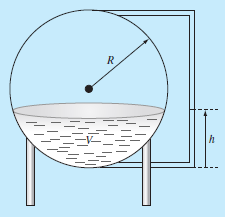
\includegraphics[scale=1]{images/Clase2-p4.png}
\end{center}}

{\problem Desarrolle un programa amigable para el usuario para el método de la falsa posición. La estructura del programa debe ser similar al pseudocódigo de la falsa posición que se bosquejó en la página 4. Pruebe el programa con la repetición del Problema 3.2.}
\end{multicols}

\end{document}

